% !TeX program = lualatex

\documentclass[12pt]{article}



\usepackage[margin=1in]{geometry} 
\usepackage{amsmath,amsthm,amssymb}
\usepackage{MnSymbol}
\usepackage{graphicx}
\usepackage{bm}
\usepackage[normalem,normalbf]{ulem}
\usepackage{algorithm} 
\usepackage{algpseudocode} 
\usepackage{multirow}
\usepackage{rotating}
\usepackage{therefore}

\usepackage{tikz}
\usetikzlibrary{shapes.multipart}
\usetikzlibrary{shapes.symbols}

\usetikzlibrary{graphs,graphdrawing,graphs.standard,quotes}
\usegdlibrary{circular,force,layered,routing}
\tikzset{
	graphs/simpleer/.style={
		nodes={draw,circle, blue, left color=blue!20, text=black, inner sep=1pt},
		node distance=2.5cm, nodes={minimum size=2em}
	},
	every loop/.style={},
}

\newcommand*\circled[1]{\tikz[baseline=(char.base)]{
		\node[shape=circle,draw,inner sep=2pt] (char) {#1};}}

\newcommand{\m}{\medskip\\}
\newcommand{\N}{\mathbb{N}}
\newcommand{\Z}{\mathbb{Z}}
\newcommand{\R}{\mathbb{R}}
\newcommand{\bbs}{\textbackslash\textbackslash\space}
\newcommand{\bs}{\textbackslash\space}
\newcommand{\la}{\enskip\land\enskip}
\newcommand{\lo}{\enskip\lor\enskip}
\newcommand{\comp}[1]{#1^\mathsf{c}}
\newcommand{\micdrop}{\qed}
\newcommand{\contra}{\begin{tikzpicture}
		\node[starburst, draw, minimum width=3cm, minimum height=2cm,line width=1.5pt,red,fill=yellow,scale=.5]
		{BOOM, A CONTRADICTION!!!};
\end{tikzpicture}}

\renewcommand{\qedsymbol}{$\blacksquare$}

\DeclareMathOperator{\lcm}{lcm}

\newtheorem{theorem}{Theorem}

\newenvironment{exercise}[2][Exercise]{\begin{trivlist}
		\item[\hskip \labelsep {\bfseries #1}\hskip \labelsep {\bfseries #2.}]}{\end{trivlist}}

\setlength\parindent{24pt}

\makeatletter
\renewcommand*\env@matrix[1][*\c@MaxMatrixCols c]{%
	\hskip -\arraycolsep
	\let\@ifnextchar\new@ifnextchar
	\array{#1}}
\makeatother
\setlength\parindent{24pt}



\begin{document}
	
	% --------------------------------------------------------------
	%                         Start here
	% --------------------------------------------------------------
	
	
	\title{Homework 5 (Due Feb 15, 2023)}
	\author{Jack Hyatt\\ %replace with your name
		MATH 575 - Discrete Mathamatics II - Spring 2023} 
	
	\maketitle
	
	Justify all of your answers completely.\\
	
	
	\medskip 
	
\begin{enumerate}

\item A {\em permutation matrix} is a square matrix with entries in $\{0,1\}$ such that each row and each column have exactly one 1. Prove that a square matrix of nonnegative integers can be expressed as a sum of $k$ permutation matrices if and only if all rows and column sums equal $k$.
\begin{proof}
	$(\implies):$\\
	Assume a square matrix of nonnegative integers can be expressed as a sum of $k$ permutation matrices. Then each of the $k$ matrices has a single 1 in each row and column. Then each sum of the rows and columns will be $1+\ldots+1$, with $k$ 1's. This equates to $k$ for each row and column.\qed\\
	$(\impliedby):$ Let us induct on all rows and columns summing to $k$.\\
	\textbf{Base Case}:$k=1$, this is already a permutation matrix, so it is a sum of 1 permutation matrix.\\
	\textbf{Induction Step}: Let $M_{n\times n}$ be a matrix whose rows and columns each sum up to $k$, for some natural number $n$. Assume $\forall k'<k$ s.t. any square matrix whose rows and columns each sum up to $k'$ be able to be expressed as a sum of $k'$ permutation matrices.\\
	Let us construct a bipartite graph $G = X\cupdot Y$, where $X = [n]$ and $Y=[n]$. $\forall x\in X,y\in Y: xy\in E(G)\iff M_{x,y}>0$. An example is below:
	\[\begin{bmatrix}[ccc]
		1 & 0 & 1 \\
		0 & 2 & 0 \\
		1 & 0 & 1
	\end{bmatrix}\]
	\begin{center}
		\tikz \graph [math nodes,grow right sep=1cm,nodes={circle,draw}]{ 
			subgraph I_nm [V={1_r,2_r,3_r}, 
			W={1_c,2_c,3_c}];
			
			1_r -- {1_c,3_c};
			2_r -- {2_c};
			3_r -- {1_c,3_c};
		};
	\end{center}
	If we can show there is a perfect matching on this graph, then there is a permutation matrix we can subtract off of the matrix, as every row will be paired with a column.\\
	Let $S\subseteq X$. Since $M$ has rows adding up to $k$, $\sum_{x\in S}\sum_{y\in Y} M_{x,y} = k|S|$. The neighborhood of $S$ will contain every column that has a positive number in any of the rows. If a column is not in the neighborhood, then it has a 0 in every row in $S$. So the columns outside of $N(S)$ do not contribute to that summation. So $\sum_{x\in S}\sum_{y\in Y} M_{x,y} = \sum_{x\in S}\sum_{y\in N(S)} M_{x,y} = k|S|$.\\
	Since $S$ is a subset of $X$, $\sum_{x\in S}\sum_{y\in N(S)} M_{x,y} \leq \sum_{x\in X}\sum_{y\in N(S)} M_{x,y}$. Since the columns add up to $k$, $\sum_{x\in X}\sum_{y\in N(S)} M_{x,y} = k|N(S)|$. So we have $k|S|= \sum_{x\in S}\sum_{y\in N(S)} M_{x,y} \leq \sum_{x\in X}\sum_{y\in N(S)} M_{x,y} = k|N(S)|$. So $k|S|\leq k|N(S)| \implies |S|\leq|N(S)|$.\\
	So by Hall's theorem, we know we can subtract off a permutation matrix from $M$. We shall call this subtracted permutation matrix $P$ and the new matrix $M'$. We have $M = P+M'$. Since $P$ is a permutation matrix, each row and column of $M'$ now adds up to $k-1$. By the induction hypothesis, we know $M'$ can be expressed as a sum of $k-1$ permutation matrices. So $M$ can be expressed as those same permutations matrices plus $P$.
\end{proof}


\medskip

\item Recall that $\alpha'(G)$ denotes the maximum size of a matching in $G$ and $\beta(G)$ denotes the minimum size of a vertex cover of $G$.
\begin{enumerate}
\item Prove that for every graph $G$, $\beta(G) \leq 2 \alpha'(G)$.
\begin{proof}
	Let $M$ be a maximum matching of $G$. For each edge in $M$, let us put both vertices incident into our vertex cover. So this vertex cover, we'll denote $C$, has size $2 \alpha'(G)$. It suffices to show that this is always a valid vertex cover. Assume towards contradiction that this is not a complete vertex cover. So then $\exists e\in E(G)$ that is not incident to any vertex in $C$. Since neither vertex incident to $e$ is in $C$, neither vertex was saturated by $M$. So we could add $e$ to $M$ and still have a matching. But $M$ was maximum, a contradiction. So $C$ is a valid vertex cover.
\end{proof}
\item For every $k \in \mathbb N$, construct a graph $G$ with $\alpha'(G) = k$ and $\beta(G) = 2k$.\m
Let us consider a graph with $k$ separate $K_3$ induced subgraphs. We know that $\alpha'(K_3)=1$ and $\beta(K_3)=2$. As our graph has $k$ many $K_3$ components, we get $\alpha'(G)=1\cdot k$ and $\beta(G)=2\cdot k$.
\end{enumerate}

\medskip


\item Matchings and vertex covers
\begin{enumerate}
\item Use the K\"onig--Egerv\'ary Theorem to prove every bipartite graph $G$ has a matching of size at least $\frac{|E(G)|}{\Delta(G)}$.
\begin{proof}
	Let $C$ be a minimum vertex cover for some graph $G$, then $$|E(G)|\leq\sum_{v\in C}d(v) \leq \sum_{v\in C}\Delta(v) = |C|\Delta(G)$$. So for any graph, $|E(G)|\leq \beta(G)\Delta(G)$. Now assume $G$ is a bipartite graph.
	\[\begin{aligned}
	&\beta(G)\Delta(G) \geq |E(G)|\\
	\iff &\alpha'(G)\Delta(G)\geq|E(G) && \text{By K\"onig--Egerv\'ary Theorem}\\
	\iff &\alpha'(G) \geq \frac{|E(G)}{\Delta(G)}
	\end{aligned}\]
\end{proof}
\item Use (a) to conclude that every subgraph of $K_{n,n}$ with more than $(k-1)n$ edges has a matching of size at least $k$.
\begin{proof}
	Let $H$ be a subgraph of $K_{n,n}$ with more than $(k-1)n$ edges. From (a), $\exists$ a matching $M$ s.t. $|M| \geq \frac{|E(G)|}{\Delta(G)}$.
	\begin{align*}
		|M| &\geq \frac{|E(G)|}{\Delta(G)}\\
		&> \frac{(k-1)n}{\Delta(G)}\\
		&\geq \frac{(k-1)n}{n} &&\text{Since } \Delta(K_{n,n})\leq n\\
		&= k-1
	\end{align*}
	So $|M|>k-1 \implies |M|\geq k$.
\end{proof}
\end{enumerate}

\medskip 
\item Recall that $\alpha(G)$ is the size of a largest independent set in $G$. 
\begin{enumerate}
\item Prove that if $G$ is an $n$-vertex bipartite graph, then $\alpha(G) \geq n/2$.\m
Since $G$ is bipartite, at least one of the bipartitions will have at least $n/2$ vertices. Just take that set and boom, we have $\alpha(G) \geq n/2$.

\item Prove that for any $n$-vertex graph $G$, $\alpha(G) \geq \frac{n}{\Delta(G)+1}$.
\begin{proof}
	Let us consider the maximum independent set. The neighborhood of the independent set is the rest of the graph, which is also a vertex cover. The maximum size the neighborhood can be is if all vertices in the independent set had a max degree, so $\alpha(G)\Delta(G)$.
	\[\alpha(G)\Delta(G)\geq\beta(G) \iff \alpha(G)\Delta(G)\geq n-\alpha(G)  \iff \alpha(G)\Delta(G)+\alpha(G)\geq n\]\[\iff \alpha(G) \geq \frac{n}{\Delta(G)+1}\]
\end{proof}
\item Show that (b) is best possible by constructing for every pair of non-negative integers $r,s$ a graph $G$ with $\alpha(G) = r$, $\Delta(G) = s$, and $\alpha(G) = \frac{n}{\Delta(G)+1}$.\m
To do this, we will need $r=\frac{n}{\Delta(G)+1}\implies n=r(s+1)$. A simple trick will be to have $G$ have $r$ different connected components, with each component having a maximum independent set of size 1. Complete graph do such a thing. The size of those complete components will then need to be $s+1$ to satisfy the number of vertices condition and the $\Delta(G)$ condition. So then $r$ connected components of $K_{s+1}$ will satisfy the desired results.
\end{enumerate}
\medskip
\item Consider the graph $G$ below.
\begin{center}
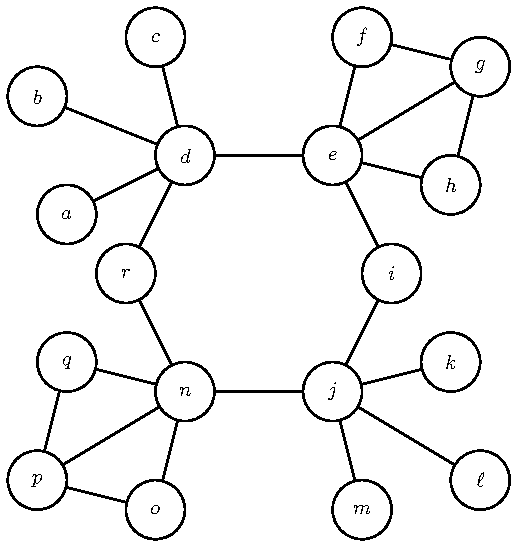
\includegraphics[scale=1]{5_2.pdf}
\end{center}
\begin{enumerate}
\item Find a matching of size $6$ in $G$.\m
Let $M = {cd,fg,eh,rn,po,jl}$.
\item Prove that your matching in part (a) is maximum using the Berge--Tutte Formula.\m
Let $S = \{d,j\}$. Then the deficiency for that set is $o(G-S)-|S| = 8-2 = 6$. $n-6 = 18-6=12$. So if $S$ is the set for the max deficiency, then the max matching will saturate 12 vertices. My matching in (a) does, so it is max.
\item Prove that your matching in part (a) is maximum using the K\"onig--Egerv\'ary Theorem.\m
Let $C = \{p,n,g,e,d,j\}$. This is a vertex cover of size 6. Since we have a vertex cover the same size of a matching, we know by strong duality that they are both optimal.
\end{enumerate}
\end{enumerate}
\end{document}
